\documentclass[10]{article}
\usepackage[margin=1in]{geometry}

\usepackage{graphicx}
\graphicspath{{./figs/}}
\usepackage{fancyvrb,color,amssymb,float,alltt,verbatim}
\usepackage{amsmath,mathtools,listings,multicol,hyperref,enumerate}
\usepackage[usenames,dvipsnames,svgnames,table,hyperref]{xcolor}

\usepackage{color}
\usepackage[backend=biber]{biblatex}
\bibliography{final_report}

\begin{document}
\begin{center}
\huge{\textbf{CS229 - Final Report}} \\
\end{center}
\begin{center}
\huge{\textbf{Predicting Political Ideology Using Campaign Finance Data}} \\
\end{center}
\begin{center}
\large{Keri A. McKiernan and Joe A. Napoli \\
\vspace{.25em}
December 12, 2015}
\end{center}
%------------------------------------------------------------------------------%
\section*{Introduction}
% Explain the problem and why it is important. Discuss your motivation for
% pursuing this problem. Give some background if necessary. Clearly state what
% the input and output is. Be very explicit: "The input to our algorithm is an
% {image, amplitude, patient age, rainfall measurements, grayscale video, etc.}.
% We then use a {SVM, neural network, linear regression, etc.} to output a
% predicted {age, stock price, cancer type, music genre, etc.}." This is very
% important since different teams have different inputs/outputs spanning
% different application domains. Being explicit about this makes it easier for
% readers. If you are using your project for multiple classes, add a paragraph
% explaining which components of the project were used for each class.

%------------------------------------------------------------------------------%
\section*{Related Work}
% You should find existing papers, group them into categories based on their
% approaches, and talk about them: Discuss strengths and weaknesses. In your
% opinion, which approaches were clever/good? What is the state-of-the-art? Do
% most people perform the task by hand? You should aim to have at least 5
% references in the related work. Include previous attempts by others at your
% problem, previous technical methods, or previous learning algorithms. Google
% Scholar is very useful for this: https://scholar.google.com/ (you can click
% "cite" and it generates MLA, APA, BibTeX, etc.)

%------------------------------------------------------------------------------%
\section*{Dataset and Features}
% Give details about your dataset: how many training/validation/test examples do
% you have? Is there any preprocessing you did? What about normalization or data
% augmentation? What is the resolution of your images? How is your time-series
% data discretized? Include a citation to where you got your dataset from.
% Depending on available space, show some examples from your dataset. You should
% also talk about the features you used. If you extracted features using Fourier
% transforms, word2vec, histogram of oriented gradients (HOG), PCA, ICA, etc.
% make sure to talk about it. Try to include examples of your data in the report
% (e.g. include an image, show a waveform, etc.).

\begin{figure}[H]
\centering
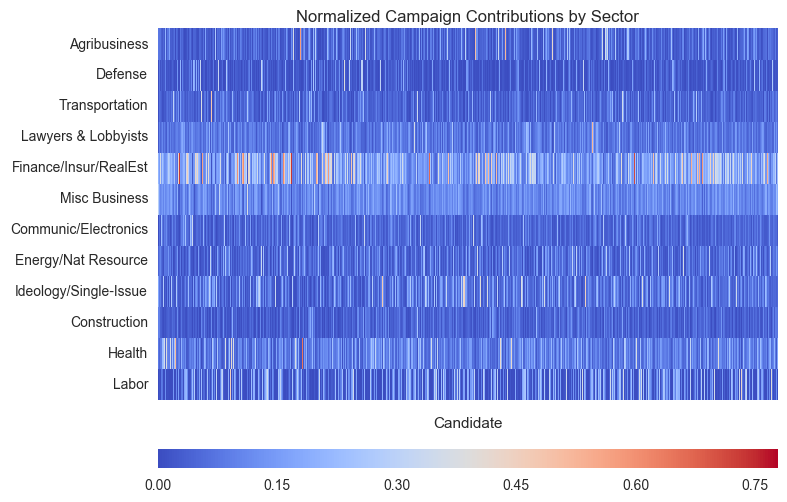
\includegraphics[width=.8\textwidth]{cand_2010_2012_2014_fm_trim_normed_feature_hm.png}
\caption{\label{fig:pc_all}Heatmap of complete feature set}
\end{figure}

%------------------------------------------------------------------------------%
\section*{Methods}
% Describe your learning algorithms, proposed algorithm(s), or theoretical
% proof(s). Make sure to include relevant mathematical notation. For example,
% include the SVM optimization objective/formula or say what the softmax function
% is. It is okay to use formulas from the lecture notes. For each algorithm, give
% a brief description (2-3 sentences) of how it works. Again, we are looking for
% your understanding of how these machine learning algorithms work. Although the
% teaching staff probably know the algorithms, future readers may not (reports
% will be posted on the class website). Additionally, if you are using a niche or
% cutting-edge algorithm (e.g. long short-term memory, SURF features, or anything
% else not covered in the class), you may want to explain your algorithm using
% several paragraphs. Note: Theory/algorithms projects may have an appendix
% showing extended proofs (see appendix description below).

%------------------------------------------------------------------------------%
\section*{Experiments/Results/Discussion}
% You should also give details about what (hyper)parameters you chose (e.g. why
% did you use X learning rate for gradient descent, what was your mini-batch size
% and why) and how you chose them. Did you do cross-validation, if so, how many
% folds? Before you list your results, make sure to list and explain what your
% primary metrics are: accuracy, precision, AUC, etc. Provide equations for the
% metrics if necessary. For results, you want to have a mixture of tables and
% plots. If you are solving a classification problem, you should include a
% confusion matrix or AUC/AUPRC curves. Include performance metrics such as
% precision, recall, and accuracy. For regression problems, state the average
% error. You should have both quantitative and qualitative results. To reiterate,
% you must have both quantitative and qualitative results! This includes
% unsupervised learning (talk with your project TA on how to quantify
% unsupervised methods). Include visualizations of results, heatmaps, examples of
% where your algorithm failed and a discussion of why certain algorithms failed
% or succeeded. In addition, explain whether you think you have overfit to your
% training set and what, if anything, you did to mitigate that. Make sure to
% discuss the figures/tables in your main text throughout this section. Your
% plots should include legends, axis labels, and have font sizes that are
% readable when printed.

%------------------------------------------------------------------------------%
\section*{Conclusion/Future Work}
% Summarize your report and reiterate key points. Which algorithms were the
% highest-performing?  Why do you think that some algorithms worked better than
% others? For future work, if you had more time, more team members, or more
% computational resources, what would you explore?

%------------------------------------------------------------------------------%
\end{document}
